\section{Finite automata for determined/undetermined systems} \label{sc:determinism}

Determinism is an important part of real time computing providing much needed predictability to the execution of tasks. When a task requires a predictable amount of computing resources, a more precise schedule can be made improving the overall performance of the system. One method for making a job deterministic is by using finite state automata. This chapter will detail deterministic and timed finite automata for exploring determinism and non-deterministic finite automata for a short discussion on non-determinism and their relationship with real-time computing. 

\subsection{Finite automata for (un)deterministic systems}

\subsection{Deterministic finite automata (DFA)}
A variant of finite automata where each state is allowed to have up to one exit transition from each state for a given member of the alphabet. This makes the execution of the automata very predictable. A DFA is considered complete if there is an exit transition for each member of the valid alphabet. 

\begin{figure}[h!]\label{}
    \centering
    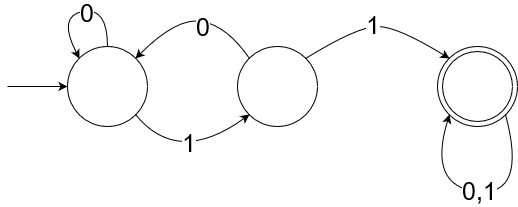
\includegraphics[scale=0.5]{realTimeComputing/fig/DFA.png}
    \caption{An DFA that accepts any input that contains two '1' symbols in a row}
    \label{fig:dfaSample}
\end{figure}

\subsection{Non-deterministic finite automata (NFA)}
A variant of finite automata where each state is allowed to have more than one exit transition for a given member of the alphabet. As a consequence the state machine can be in multiple states simultaneously and will continue running until any path reaches an end-state. This unpredictability makes the automaton highly volatile with regards to execution time, and therefore illsuited for time sensitive execution.\par

Any NFA can be converted into a DFA using an algorithm known as powerset construction.

\subsection{Timed finite automata (TFA)}
A variant on DFA where in addition to the input stream, there are defined clocks. Clocks can be reset on transitions, and the machine can only be in a local variant of a state for as long as the indicated clock values are fulfilled. As in DFA the TFA is always waiting for the next symbol before continuing, but in addition to the datastream the model can use clock values as switch triggers. For a switch to occur the next symbol must arrive before the time is up, otherwise the execution will be rejected. 

\begin{figure}[h!]\label{}
    \centering
    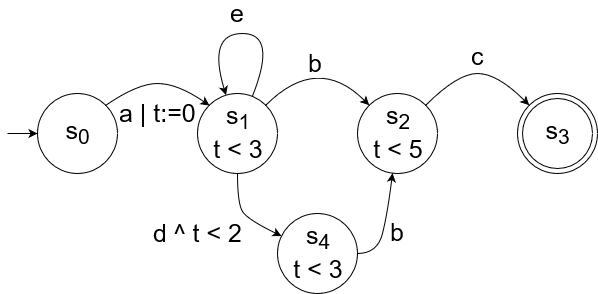
\includegraphics[scale=0.5]{realTimeComputing/fig/TFA.png}
    \caption{A sample TFA}
    \label{fig:tfaSample}
\end{figure}

In the TFA shown on figure \ref{fig:tfaSample}, the control will go from s_0 to s_1 when 'a'. In s_1 it can take any number of 'e' as long as t < 3. From s_1 it is possible to go to s_4 on 'e' as long as t < 2. From s_1 or s_4 control can be passed to s_2 on 'b' which must happen before t = 3. Finally control will be passed to s_3 on 'c' before t = 5.

\subsection{Compare deterministic and non-deterministic automata}
The difference between deterministic and non-deterministic automata lies in their focus of execution, with NFA the execution is operated as a sort of breadth first search algorithm as the execution spreads through the entire automata searching for an end state. DFA on the other hand will only ever operate in a single state and are therefore more manageable and predictable. When it comes to realtime computing, predictability is king.

\subsection{Talk about timed automata and how they comply with deadlines}
By adding clocks to deterministic automata the state machine gains the concept of time, which is neccessary to make any requirements regarding deadlines. By setting time limits to how long an execution can run the programmer can, during implementation, be aware of and work within the required time frames for each given state. This quantification of the available resources allows the system to utilize it's resources to the limit, while also staying sufficiently responsive. 

